\documentclass[11pt, oneside]{article}   	% use "amsart" instead of "article" for AMSLaTeX format
\usepackage{geometry}                		% See geometry.pdf to learn the layout options. There are lots.
\geometry{letterpaper}                   		% ... or a4paper or a5paper or ... 
%\geometry{landscape}                		% Activate for for rotated page geometry
%\usepackage[parfill]{parskip}    		% Activate to begin paragraphs with an empty line rather than an indent
\usepackage{graphicx}				% Use pdf, png, jpg, or eps� with pdflatex; use eps in DVI mode
								% TeX will automatically convert eps --> pdf in pdflatex		
\usepackage{amssymb}
\usepackage{amsmath}
\usepackage{parskip}
\usepackage{color}
\usepackage{hyperref}

\title{Complex numbers, functions and calculus}
%\author{The Author}
%\section{}
%\subsection*{}
\date{}							% Activate to display a given date or no date

\graphicspath{{/Users/telliott_admin/Dropbox/Tex/png/}}
% \begin{center} 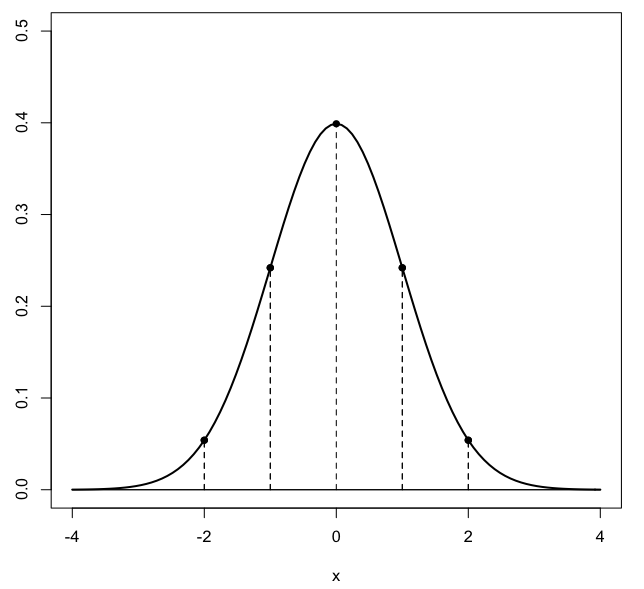
\includegraphics [scale=0.4] {gauss3.png} \end{center}
\begin{document}
\maketitle
\Large
\section{Complex numbers}

You undoubtedly know that complex numbers arise in the context of finding solutions to certain polynomials, for example, this equation:
\[ x^2 + 1 = 0 \]
which has no solution among the real numbers.  

It is easy to see why, since $x^2$ is $\ge 0$ for all $x \in \mathbb{R}$, so adding $1$ to $x^2$ cannot bring the sum back to zero.  

Visualizing the same function geometrically, this is just the simple parabola $y=x^2$ shifted up, moving its vertex from $(0,0)$ to $(0,1)$.  A plot shows that the graph of the function never crosses the $x$-axis---there are no values on the curve and on the line $x=0$.

Now, define $i = \sqrt{-1}$, so that $i^2 = -1$, which gives $\pm \ i$ as the solutions to the above equation.  

Having $i$ available, any square root like $\sqrt{-a^2}$, where $a$ is a real number, can be factored as $\sqrt{-1} \ \sqrt{a^2} = ia$.

However, note that the converse is not necessarily true.  Consider
\[ i^2 = \sqrt{-1} \cdot \sqrt{-1} \stackrel{?}{=} \sqrt{(-1)\cdot (-1)} = \sqrt{1} \]

Now, $\sqrt{1}$ has two solutions $ \pm \ 1$, and we normally choose the positive root when thinking about $\sqrt{x}$ as a \emph{function}.  But $i^2$ is equal to $-1$ not $1$.  What's the deal?

The equality with a question mark is not valid
\[ \sqrt{-1} \cdot \sqrt{-1} \ne \sqrt{(-1)\cdot (-1)} \]

which explains why this "proof" is erroneous.

We consider complex numbers $z$ as combinations like
\[ z = a + ib \]
 where $a$ and $b$ are both real numbers.  $a$ is called the real part, and $b$ is called the imaginary part of the complex number $z$.

In the example above, it is not true that
\[ \sqrt{a} \cdot \sqrt{b} = \sqrt{ab} \]
when both terms are purely imaginary numbers.

Some useful identities involving $i$ include
\[ i^2 = -1 \]
\[ i = -\frac{1}{i} \]
\[  -i = \frac{1}{i} \]

For much of what is done with complex numbers the fact that $i$ equals $\sqrt{-1}$ is not relevant.

Instead, we simply have ordered pairs of real numbers $(a,b)$ and the $i$ notation is a bookkeeping device, a marker to remind us that when we multiply
\[ (a + ib) (c + id) \]
the last term is
\[ ib \cdot id = -bd \]
The result of multiplying $ib \cdot id$ is a real number with the sign flipped, while a real number $a$ times an imaginary number $id$ is equal to $iad$ and
\[ (a + ib) (c + id) = ac -bd + i(ad + bc) \]

In other words, a complex number is simply an \emph{ordered pair} such as $(a,b)$.  

Note carefully that if we consider two complex numbers $z_1 = a + ib$ and $z_2 = c + id$, then 
\[ z_1 = z_2 \iff a = c \text{ and } b = d \]
If and only if both the real and the imaginary parts are equal, then the two complex numbers $z_1$ and $z_2$ are equal.

Another way to keep track of the same information is in matrix form, namely:
\[
\begin{bmatrix}
a & -b \\
b &  \ \ a
\end{bmatrix}
\]
Such matrices can be added and multiplied in the normal way and give the desired results for complex numbers.  Thus:
\[
\begin{bmatrix}
a & -b \\
b &  \ \ a
\end{bmatrix} \times
\begin{bmatrix}
c & -d \\
d &  \ \ c
\end{bmatrix} =
\begin{bmatrix}
ac + bd & -ad - bc \\
ad + bc &  \ \ ac + bd
\end{bmatrix} 
=
\begin{bmatrix}
 u & -v \\
v &  \ \ u
\end{bmatrix}
\]
Yet another way to think about complex numbers is to use the complex plane (the Argand plane), where points are plotted with the real part along the horizontal axis and the imaginary part along the vertical axis.

Looking at the graphic, the distance of any point from the origin is equal to $r$, and $\theta$ is the angle the ray makes with the positive $x$-axis in a CCW direction.  

This figure and the next two are from Brown.
\begin{center} 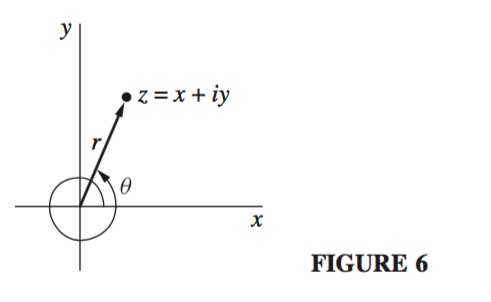
\includegraphics [scale=0.6] {Brown6.png} \end{center}

Switching notation to
\[ z = x + iy \]
for the complex number $z$ we have
\[ x = r \cos \theta \]
\[ y = r \sin \theta \]
\[ x + iy = r \cos \theta + ir \sin \theta\]
\[ = r(\cos \theta + i \sin \theta) \]
\[ = re^{i\theta} \]
where the last part makes use of Euler's famous equation.  $r$ is called the \textbf{modulus} and $\theta$ is called the \textbf{argument} or \textbf{phase}.

Notice that in the figure above the argument $\theta$ is actually $\theta + 2 \pi$.  All multiples $2k \pi$ for $k \in 0, \pm 1, \pm 2 \dots$ are valid.

Calculations may be easier using one form rather than another.  Addition is simpler with $a + ib$ (the Cartesian format), while multiplication is better with the polar format.  Matrices are fine for both addition and multiplication.
 
Here is multiplication in polar coordinates
\[ r e^{i\theta} \ \rho e^{i\phi} = r \rho \ e^{i (\theta + \phi)} \]
and 
\[ (r e^{i\theta})^2 = r^2 e^{i2\theta} \]

Multiplication of $z_1 = r e^{i\theta}$ by $z_2 = \rho e^{i\phi}$ stretches $r$ (the length of $z_1$) by the factor $\rho$ (the length of $z_2$), and rotates $z_1$ by adding a phase shift of $\phi$ to the original angle $\theta$.
\begin{center} 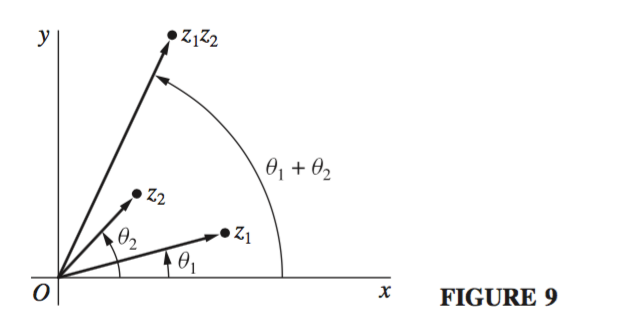
\includegraphics [scale=0.6] {Brown9.png} \end{center}

\subsection*{complex conjugate}
The complex conjugate of
\[ z = x + iy \]
is
\[ z* = x - iy \]

The complex conjugate of $z$ is also written as $\bar{z}$.

The \emph{length} of $z$ squared is
\[ zz* = (x + iy) (x - iy) \]
\[ = x^2 + y^2 \]
\[ = r^2 \cos^2 \theta + r^2 \sin^2 \theta \]
\[ = r^2   \]
Again, $r$ is the length of the ray from the origin to $z$ as plotted in the complex plane.
\[ r = \sqrt{zz*} \]
The point corresponding to $z*$ in the complex plane has the same overall distance from the origin and the same $x$-component as $z$, but the sign change on $y$ means that $z*$ is reflected across the $x$-axis from $z$.
\begin{center} 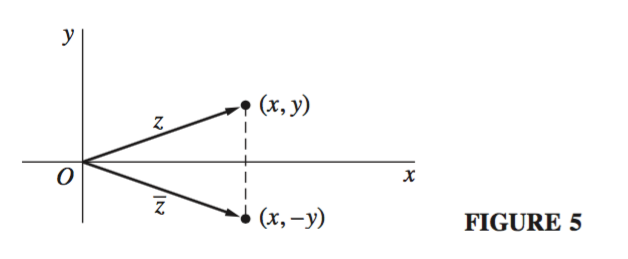
\includegraphics [scale=0.6] {Brown5.png} \end{center}

In polar coordinates, if $z = re^{i \theta}$ then $z* = re^{i (- \theta)} = re^{-i\theta}$.  So
\[ zz* = re^{i \theta} \ re^{i - \theta} = r^2 e^0 = r^2 \]
Alternatively
\[ (x + iy)(x - iy) = x^2 - ixy + ixy -i^2y^2 \]
\[ = x^2 + y^2 \]
The value of $z$ multiplied by its complex conjugate $z*$ is equal to the square of the length $r$.  Multiplication by $z*$ makes the product entirely real.  

If we consider addition rather than multiplication of the complex conjugate we observe that it also gives an entirely real result:
\[ z + z* = x + iy + x - iy = 2x \]
while subtraction gives an entirely imaginary result:
\[ z - z* = x + iy - x + iy = i2y \]

Using the complex conjugate is the best way to deal with the inverse function (or with division by a complex number):
\[ \frac{1}{z} = \frac{z*}{zz*} = \frac{a - ib}{a^2 + b^2} \]
or in polar notation:
\[  \frac{1}{z} =  \frac{r e^{-i \theta}}{r^2 \ e^{i \theta} \ e^{-i \theta}} = \frac{1}{r} \ e^{-i \theta} \]

Let's think about what it means to take the inverse for different $z$.  In every case, the point is reflected across the $x$-axis (the ray makes an angle $- \theta$ with the $x$-axis).  

There is no change in length for $r=1$.  But if say 
\[ z = 1 + i = (1,1) = \sqrt{2} \ e^{i \cdot \pi/4} \]
then the new point has $r = \frac{1}{\sqrt{2}}$ and it is at
\[ \frac{1}{z} = \frac{1}{\sqrt{2}} e^{-i \cdot \pi/4} = (\frac{1}{2},- \frac{1}{2}) = \frac{1}{2} - i \frac{1}{2}\]

Another result (that we won't prove right now) is that if we have an expression involving several complex numbers:
\[ w = f(z_1, z_2 \dots) \]
we can obtain the complex conjugate of the whole thing by substituting the complex conjugate of each component:
\[ w* = f(z_1*, z_2* \dots) \]

\subsection*{complex functions:  roots}
Consider the function $\sqrt{z}$.  Now, for the modulus part, $\sqrt{r} \cdot \sqrt{r}$ is obviously equal to $r$, and what we need to do for the argument is to find an angle that is one-half of the original one, which leads us to
\[ \sqrt{z} = \sqrt{re^{i\theta}} = \sqrt{r} \ e^{i \theta/2} \]

However, recall from trigonometry (and what we said above) that $\theta + 2k \pi$ is the same angle as $\theta$, for integer $k$ ($k \in \mathbb{Z}$).

The same thing is true here.  It is allowed that $\theta' = (2k \pi + \theta)$ for $k \in \{ 0, \pm 1, \pm 2 \dots \}$, since the result maps to the same point in the plane.

This means that a second solution to the square root problem is
\[ \sqrt{re^{i\theta}} = \sqrt{r} \ e^{i (\pi + \theta/2)} \]
because, again, $\sqrt{r} \cdot \sqrt{r} = r$ and
\[ \ e^{i (\pi + \theta/2)} \cdot \ e^{i (\pi + \theta/2)} = e^{i (2\pi + \theta)} = e^{i\theta} \]

For the square root, there is only one additional distinct solution, since one-half of $4 \pi + \theta = 2 \pi + \theta/2$ which is no different than $\theta/2$, but the cube root has 3 solutions and in general the $n^{th}$ root has $n$ solutions.

Consider points on the unit circle with $r=1$ (so $\sqrt{r} = r$) and suppose
\[ \theta = \pi/2 \]
so
\[ z = e^{i \pi/2} \]
Points with $\theta = \pi/2$ lie directly above the origin on the imaginary axis (there is no real component).  This point is one unit from the origin so it is the point $(0 + i \cdot 1) = i$.  Thus
\[ e^{i \pi/2} = i \]
Note that
\[ (e^{i \pi/2})^2 = e^{i (\pi/2 + \pi/2)}\]
\[ = e^{i\pi} = -1 = i^2 \]

$\sqrt{e^{i \pi/2}} = \sqrt{i}$ has two possible values.  One is
\[ \sqrt{e^{i\pi/2}}  = (e^{i\pi/2})^{1/2} = e^{i\pi/4} \]
Let's just check.  The point is at a distance $1$ from the origin and angle $\theta = \pi/4$.  We go equal distances along the real and imaginary axes:
\[ x = \cos \theta = \frac{1}{\sqrt{2}} \]
\[ y = \sin \theta = \frac{1}{\sqrt{2}} \]
So we have that the square is:
\[ (\frac{1}{\sqrt{2}} + i \frac{1}{\sqrt{2}} )^2 = \frac{1}{2} - \frac{1}{2} + 2 i \frac{1}{2} \]
\[ = 0 + i = i \]
the second solution is
\[ \sqrt{e^{i\pi/2}}  = e^{i \cdot 5/4 \pi} \]
which can be plotted as
\[ x = \cos \theta = -\frac{1}{\sqrt{2}} \]
\[ y = \sin \theta = -\frac{1}{\sqrt{2}} \]
The square is the same except the first term is $(- 1/\sqrt{2})^2$, so the result is unchanged.  It's a bit counter-intuitive that squaring a number may possibly reduce the phase angle, but you can think of it as modular arithmetic (mod $2 \pi$).

In general, if we're working with the complex number
\[ re^{i\theta} \]
and we want the nth root, the modulus is just
\[ \rho = r^{1/n} \]
And the question always is, what's the angle?
\[ \phi = \frac{\theta + 2k\pi}{n}, \ \ \ k = 0, 1, 2 \dots n-1 \]

Let's say we want the cube roots of $1$.  Obviously, all the roots will have length $1$.  What about the angles?  The starting angle $\theta = 0$, so $\phi = 2k\pi/3$ and 
\[ \phi_ 1= \frac{2 \pi}{3} \]
\[ \phi_2 = \frac{4 \pi}{3} \]
\[ \phi_3 = \frac{6 \pi}{3} = 0 \]
Notice that the first and second roots are complex conjugates because
\[ \phi_1 + \phi_2 = \frac{6\pi}{3} = 2 \pi = 0 \]

Suppose our number is $z = -8i$ and we want the cube roots.  Writing the number in polar coordinates:
\[ z = 8e^{3\pi/2} \]
All of the roots have the same modulus, $2$, since $2^3 = 8$.  The are three roots which differ in their arguments.  Since $\theta = 3 \pi / 2$, these are:
\[ \phi_1 = \frac{\theta}{3} = \frac{\pi}{2} \]
\[ \phi_2 = \frac{\theta + 2\pi}{3} = \frac{\pi}{2} + \frac{2\pi}{3} = \frac{5\pi}{6} \]
\[ \phi_3 = \frac{\theta + 4\pi}{3} = \frac{\pi}{2} + \frac{4\pi}{3} = \frac{7\pi}{6} \]
Notice that the second and third roots are complex conjugates.

\subsection*{Nahin's puzzle}
In one of his books Nahin starts by posing this question:  suppose we are given that 
\[ x + \frac{1}{x} = 1 \]
\emph{Without computing} $x$, find the value of
\[ x^7 + \frac{1}{x^7} \]
Nahin says that if you are the type to just start right in trying to figure this out, then you will like his book.

From its placement in this section, you might just guess the answer.  First of all, no real $x$ solves the equation
\[ x + \frac{1}{x} = 1 \]
as you will see if you use the quadratic formula.  So let's change nomenclature and call it $z$.  (Of course, we were not supposed to \emph{compute} $z$).

We may guess that $z$ is a complex number with length $1$ so that the lengths don't change with powers or roots.  

Then, all that happens is that $\theta$ changes in such a way that 
\[ 7 \theta = \theta = \frac{\theta}{7}  \]

To actually compute $z$, multiply by $z$, rearrange, and solve:
\[ z^2 + 1 = z \]
\[ z^2 - z + 1 = 0 \]
From the quadratic equation:
\[ z = \frac{1 \pm \sqrt{1 - 4}}{2} = \frac{1}{2} \pm i \frac{\sqrt{3}}{2}  \]
The square of the length is
\[ r^2 = zz* \]
\[ = (\frac{1}{2} + i \frac{\sqrt{3}}{2}) (\frac{1}{2} - i \frac{\sqrt{3}}{2})  \]
\[ = \frac{1}{4} + \frac{3}{4} = 1 \]
The angle we seek has tangent equal to $1/\sqrt{3}$.  You may recognize the sine and cosine of $\pi/3$ as the real and imaginary components of $z$.

So if 
\[ z = e^{i \pi/3} = (\frac{1}{2} + i \frac{\sqrt{3}}{2}) \]
\[ \frac{1}{z} = e^{-i \pi/3} = (\frac{1}{2} - i \frac{\sqrt{3}}{2}) \]
then when doing the addition the imaginary parts of $z$ cancel and we have that 
\[ z + \frac{1}{z} = \frac{1}{2} + \frac{1}{2} = 1 \]

The other special attribute of this value for $z$ is that the length is $1$ so all powers of $r$ are $1$.  As for the angle, $\pi/3$ is special in that $7 \times \pi/3 = 2 \pi + \pi/3 = \pi/3$.  Now it's not strictly true that \emph{the} 7th root of $\theta$ is equal to $\theta$ (since there are 7 distinct roots).  But I hope you can see that there is at least one such root.

\subsection*{powers:  de Moivre's formula}
Let $n$ be an integer:
\[ z^n = (re^{i\theta})^n = r^n e^{in\theta} \]
Suppose $r=1$:
\[ z^n = e^{in\theta} = \cos n \theta + i \sin n \theta \]
\[ (\cos \theta + i \sin \theta)^n = \cos n \theta + i \sin n \theta \]
This is de Moivre's formula.

Suppose $n=2$, then
\[ (\cos \theta + i \sin \theta)^2 \]
\[ = \cos^2 \theta - \sin^2 \theta + i\ 2 \sin \theta \cos \theta \]
Equating with the right-hand side of de Moivre's formula:
\[ \cos^2 \theta - \sin^2 \theta + i\ 2 \sin \theta \cos \theta = \cos 2 \theta + i \sin 2 \theta \]
we find that
\[ \cos 2 \theta = \cos^2 \theta - \sin^2 \theta \]
\[ \sin 2 \theta = 2 \sin \theta \cos \theta \]
We already know these, they are the double angle formulas.

Suppose $n=3$, then
\[ (\cos \theta + i \sin \theta)^3 \]
\[ = \cos^3 \theta - 3 \cos \theta \sin^2 \theta + i (3 \cos^2 \theta \sin \theta - \sin^3 \theta) \]
we find that
\[ \cos 3 \theta =\cos^3 \theta - 3 \cos \theta \sin^2 \theta \]
\[ \sin 3 \theta = 3 \cos^2 \theta \sin \theta - \sin^3 \theta \]
and so on.

We can just check that last one for $\theta = \pi/6$:
\[ \sin 3 \theta = 3 \cos^2 \theta \sin \theta - \sin^3 \theta \]
\[ 1 = 3 (\frac{\sqrt{3}}{2})^2 \ \frac{1}{2} - (\frac{1}{2})^3 \]
Multiply both sides by $2^3$:
\[ 8 = 3 (\sqrt{3})^2 - 1 \]
That looks correct.

\section{Complex functions}
The theory of complex functions ($f(z)$ where  $z \in \mathbb{C}$) is often described as being very beautiful, and in addition it makes possible the solution of many difficult integrals (over the real numbers).

Marsden gives three examples that he says are either very difficult or impossible if we cannot use complex integrals:
\[ \int_0^{\infty} \frac{\sin^2 x}{x^2} \ dx = \frac{\pi}{2} \]
\[ \int_0^{\infty} \frac{x^{\alpha-1}}{1+x} \ dx = \frac{\pi}{\sin \alpha \pi} \]
\[ \int_0^{2 \pi} \frac{d \theta}{a + \sin \theta} = \frac{2 \pi}{\sqrt{a^2-1}} \]

In this section we'll  look at some simple complex functions---just ignore the contradiction  :)

A complex function is a function whose input is a complex number $z$, an \emph{ordered pair} of two real numbers $x$ and $y$.  $f(z)$ generates or emits a second complex number which we may call $w$.
\[ w = f(z) = u(x,y) + i v(x,y) \]

The real part of $w$ is the output of $u(x,y)$, as the notation says.  It is a function of both $x$ and $y$, and similarly the imaginary part of $w$ is the output of $v(x,y)$.  The two functions $u$ and $v$ are real functions of two real variables.

Part of the "complexity" of complex functions is the multiple values of arguments, but another part of what is going on is that calculus of complex functions is not like calculus of real functions.  We're used to thinking of the derivative as a slope, but for complex functions there is no simple geometric interpretation.  The derivative maps $z$ to a new complex number, often called $w$. 

We compute the derivative of a real function as
\[ \frac{df}{dx} = \lim_{h \rightarrow 0} \frac{f(x+h) - f(x)}{h} \]
(provided this limit exists).

In "approaching" $x$ or considering $x+h$ there are only two directions, from above and from below.

For a complex function $f(z)$ which produces a complex number $w = f(z)$, the basic definition of the derivative is the same, but we may approach $z$ in the Argand plane from any one of an infinite number of directions.  The resulting change in $f(z)$ (the derivative) must then be the same for \emph{all} of them.  Not all functions have this property.  Those that do are called \emph{analytic}.

\begin{center} 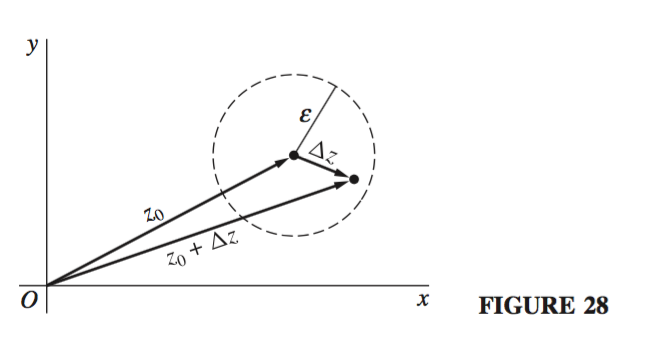
\includegraphics [scale=0.6] {Brown28.png} \end{center}

As we'll see later, if (and only if) the partial derivatives meet these conditions (called the CRE conditions):
\[ u_x = v_y \]
\[ u_y = - v_x \]
then the function in question is said to be analytic.

The technical definition of an analytic function, or analyticity, is somewhat different but this property follows from it.  We don't need to worry about the distinction.

An analytic function is differentiable, in other words, it's a good function and we can do calculus with it.  If a complex function is analytic, its derivative exists:  its value is independent of the direction in which change occurs.

So for example if we change a little bit in the $x$ direction (in a direction parallel with the real axis, with $\Delta y = 0$), we get:
\[ f'(z) = u_x + iv_x  \]

Suppose
\[ f(z) = z^2 \]
\[ = (x + iy)(x + iy) \]
\[ = x^2 - y^2 + 2ixy \]
Then
\[ f'(z) = u_x + iv_x \]
\[ = 2x + 2iy \]
\[ = 2z \]
which should not be surprising.  However, this depends on the fact that $z^2$  is an analytic function (in fact, all powers of $z$ are analytic).

There are a few functions that are important and not analytic.  These can generally be seen to involve the complex conjugate:
\[ |z|^2 = zz* \]

For functions that have a derivative everywhere (excepting points where the function may vanish, like the origin for $1/z$), most of the usual rules of calculus apply
\[ \frac{d}{dz} c = 0, \ \ \  \text{where $c$ is a constant} \]
\[ \frac{d}{dz} z = 1 \]
\[ \frac{d}{dz} z^n = nz^{n-1}, \ \ \ n \ne 0 \]
\[ (f + g)' = f' + g' \]
\[ (fg)' = f' g + f g' \]
\[ (\frac{f}{g})' = \frac{f' g - f g'}{g^2} \]

\subsection*{exponential}
For a non-trivial introduction to using the CRE, we will explore the complex exponential function $f(z) = e^z$.  First of all, write
\[ e^z = e^{x + iy} \]
\[ = e^x e^{iy} \]
We can thus visualize the complex exponential as resulting in a number $w$ with modulus $e^x$ and argument $y$.

Reversing Euler:
\[ = e^x (\cos y + i \sin y) \]
\[ = e^x \cos y + i e^x \sin y \]
So the real part of $e^z$ is 
\[ u(x,y) = e^x \cos y \]
with partial derivatives:
\[ u_x = e^x \cos y \]
\[ u_y = - e^x \sin y \]
and the imaginary part is
\[ v(x,y) = e^x \sin y \]
with partials:
\[ v_x = e^x \sin y \]
\[ v_y = e^x \cos y \]
Hence
\[ u_x = v_y \]
\[ u_y = - v_x \]
The CRE conditions are satisfied and the complex exponential $e^z$ is analytic.  (Which, according to Shankar, we could have predicted, since it depends only on $z$ and not on $z*$).

Notice also that, evaluating the derivative along $\Delta y =0$:
\[ f'(z) = u_x + iv_x  \]
\[ = e^x \cos y + i e^x \sin y = z \]
The complex exponential is its own derivative.

Which is good because we want our definitions for the complex functions to give the standard results when $z$ has only a real part, i.e. when $y=0$.

Now, once more we recall Euler's formula (for a real variable $\theta$ or $x$):
\[ e^{i \theta} = \cos \theta + i \sin \theta \]
\[ e^{i x} = \cos x + i \sin x \]
Substitute $-x$ for $x$:
\[ e^{-i x} = \cos -x + i \sin -x \]
\[ = \cos x - i \sin x \]
By addition and subtraction we obtain:
\[ 2 \cos x = e^{i x} + e^{-i x} \]
\[ \cos x = \frac{e^{i x} + e^{-i x}}{2} \]
and
\[ 2i \sin x = e^{i x} - e^{-i x} \]
\[ \sin x = \frac{e^{i x} - e^{-i x}}{2i} \]
These can be taken as the \emph{definitions} of the complex sine and cosine.

We will also need the hyperbolic sine and cosine later so let's just remind ourselves:
\[ 2 \cosh x = e^x + e^{-x} \]
\[ 2 \sinh x = e^x - e^{-x} \]

As mentioned, the derivative of the complex exponential is as we would hope and expect:
\[ \frac{d}{dz} e^z = e^z \]

This can also be proved by using a Taylor series.  Shankar says to define $e^z$ in the same way as $e^x$.  That is, for real $x$:
\[ e^x = \sum_0^{\infty} \frac{x^n}{n!} \]
which we know converges because
\[ |x| < R = \lim_{n \rightarrow \infty} \frac{|a_n|}{|a_{n+1}|} \]
where $a_n = 1/n!$.  So
\[ e^z = \sum_0^{\infty} \frac{z^n}{n!} \]
and again we see that 
\[ \frac{d}{dz} \ e^z = e^z \]
differentiating the series term by term.

The complex exponential 
\[ e^z = e^x e^{iy} \]
has some properties that are not shared with the real exponential.  As we saw before, the angle $\theta + 2 \pi = \theta$, so any number is really a family of numbers with different $\theta + 2 \pi k$ for integer $k$.

In particular, $e^z$ is periodic with a period of $2 \pi i$.  Additionally, it is possible for $e^z$ to be negative.  
\subsection*{example:  exp(z) = -1}
Let us find $z$ such that:
\[ e^z = -1 \]
This corresponds to the point $(-1,0)$.  The simplest way is to use polar coordinates.  We can see that the length is $r = 1$, and the angle $\theta$ is equal to $\pi$.  So the number is
\[ 1 \cdot e^{i\pi} = e^{i\pi} = -1 \]
Going through $x$ and $y$:  let $z = 0 + i\pi$.  Then 
\[ e^x = e^0 = 1 \]
and
\[ e^{iy} = e^{i\pi} = -1 \]
So
\[ e^z = e^x e^{iy} = e^x(\cos y + i \sin y) = 1 (-1) = -1 \]
\subsection*{example: exp(z) = i}
This corresponds to the point $(0,1)$.  We can see (again) that the length is $r = 1$, and the angle is equal to $\pi/2$.  So the number is
\[ e^{i \cdot \pi/2} = i \]
\subsection*{non-zero}
On the other hand, $e^z$ \emph{cannot be zero}.
\[ e^z = e^x \cos y + i e^x \sin y = e^x(\cos y + i \sin y) \]
For $x \in \mathbb{R}$, $e^x > 0$ so the only way this could be zero would be if we can find a $y$ such that $\sin y$ and $\cos y$ were both zero.  Since there is no such $y$, we conclude that $e^z$ cannot be equal to zero.

\subsection*{derivation of the Cauchy-Riemann equations}
For a complex function $f(z)$ which produces a complex number $w = f(z)$, we may approach $z$ in the Argand plane from any one of an infinite number of directions.

The CRE are necessary and sufficient conditions such that the derivative is the same for any direction of approach.

Here are two quick proofs in the forward direction (differentiability implies the CRE):

Write the basic definition of the derivative of $f$ at the point $z_0$:
\[ f'(z_0) = \lim_{\Delta z \rightarrow 0} \frac{f(z + z_0) - f(z)}{\Delta z} \]
Now
\[ f'(z_0) =  \frac{dw}{dz} =   \lim_{\Delta z \rightarrow 0} \frac{\Delta w}{\Delta z} \]
\[ =  \lim_{\Delta z \rightarrow 0} \frac{\Delta u + i \Delta v}{\Delta x + i \Delta y} \]
Our constraint is that the derivative must be the same for any direction of approach.  

Pick two convenient directions:  with $\Delta y = 0$ or with $\Delta x = 0$.  For the first one, we have
\[ f'(z_0) = \lim_{\Delta z \rightarrow 0} \frac{\Delta u + i \Delta v}{\Delta x + i \Delta y} \]
\[ =  \lim_{\Delta x \rightarrow 0} \frac{\Delta u + i \Delta v}{\Delta x} \]
\[  =  \lim_{\Delta x \rightarrow 0} \frac{\Delta u}{\Delta x} + i \frac{\Delta v}{\Delta x} \]
Notice that $\Delta z \rightarrow 0$ becomes $\Delta x \rightarrow 0$ (because $\Delta y = 0$) and the limit is just equal to 
\[ f'(z_0) = u_x + i v_x \]
This is a standard limit for two real functions of two real variables.

For the second approach, with $\Delta x = 0$, we have
\[ f'(z_0) =  \lim_{\Delta y \rightarrow 0} \frac{\Delta u + i \Delta v}{i \Delta y} = \lim_{\Delta y \rightarrow 0} \frac{\Delta u}{i \Delta y} +  \frac{i \Delta v}{i \Delta y} \]
Here, the $i$ terms cancel on the right (and recall that $1/i = -i$) so we have:
\[ f'(z) = -i u_y + v_y \]
Equating the two results we have that 
\[ f'(z) = u_x + i v_x = v_y - i u_y \]
Both the real and the imaginary parts must be equal:
\[ u_x = v_y \]
\[ v_x = - u_y \]
These are the CRE.
\subsection*{alternative derivation}
Write:
\[ z = x + iy \]
Clearly,
\[ \frac{\partial z}{\partial x} = 1, \ \ \ \frac{\partial z}{\partial y} = i \]
Now,
\[ w = f(z) = u(x,y) + i \ v(x,y) \]
where $u$ and $v$ are real functions over $\mathbb{R}^2$.

Recalling the chain rule
\[ w = u(x,y) + i \ v(x,y) \]
\[ \frac{\partial w}{\partial x} = \frac{dw}{dz} \ \frac{\partial z}{\partial x} \]
\[ =  \frac{dw}{dz} \]
(by the result for $\partial z/\partial x$ immediately above).
Similarly
\[ \frac{\partial w}{\partial y} = \frac{dw}{dz} \ \frac{\partial z}{\partial y} \]
\[ =  i \frac{dw}{dz} \]
\[  \frac{dw}{dz} = -i \ \frac{\partial w}{\partial y} \]
Hence we can equate the two expressions 
\[ \frac{dw}{dz} = \frac{\partial w}{\partial x} = -i \frac{\partial w}{\partial y} \]

Now if we actually compute the partials
\[ \frac{\partial w}{\partial x} = u_x + i v_x \]
\[ \frac{\partial w}{\partial y} = u_y + i v_y \]
and plug them in to the previous equation, we obtain:
\[ u_x + i v_x = -i (u_y + i v_y) = v_y - i u_y \]
Exactly as we obtained by the first approach.  And since both the real and the imaginary parts must be equal:
\[ u_x = v_y \]
\[ v_x = - u_y \]
These are the CRE, again.

The result above
\[ \frac{df}{dz} = \frac{\partial f}{\partial x} = - i \frac{\partial f}{\partial y} \]
is just saying that the derivative $df/dz$ can be computed with constant $y$, or constant $x$ or anything in between.  Take the first direction, constant $y$:
\[ \frac{df}{dz} = \frac{\partial f}{\partial x} = u_x + i v_x \]

From above
\[ u_x = e^x \cos y \]
\[ v_x = e^x \sin y \]
\[ \frac{df}{dz} = \frac{\partial f}{\partial x} =  e^x \cos y + i  e^x \sin y = z \]
Just like for $x \in \mathbb{R}$, where
\[ \frac{d}{dx} \ e^x = e^x \]
For a $z \in \mathbb{C}$
\[ \frac{d}{dz} \ e^z = e^z \]

\subsection*{polar coordinates}

An alternative form of the CRE holds in polar coordinates:
\[ r u_r = v_{\theta} \]
\[ u_{\theta} = - r v_r \]

One way to get this is to write
\[ \frac{\partial u}{\partial r} =  \frac{\partial u}{\partial x}\frac{\partial x}{\partial r} + \frac{\partial u}{\partial y}\frac{\partial y}{\partial r} \]
and since 
\[ z = x + iy \]
\[= r \cos \theta + r \sin \theta \]
then using the equation with the partials and computing $x_r$, $y_r$ etc.:
\[ u_r = u_x x_r + u_y y_r \]
\[ u_r = u_x \cos \theta + u_y \sin \theta \]
while
\[ u_{\theta} = u_x x_{\theta} + u_y y_{\theta} \]
\[ u_{\theta} = -u_x \ r \sin \theta + u_y \  r \cos \theta \]
similarly
\[ \frac{\partial v}{\partial \theta} =  \frac{\partial v}{\partial x}\frac{\partial x}{\partial \theta} + \frac{\partial v}{\partial y}\frac{\partial y}{\partial \theta} \]
\[ v_{\theta} = -v_x \ r \sin \theta + v_y \ r \cos \theta \]
while
\[ v_r = v_x x_r + v_y y_r \]
\[ v_r = v_x \cos \theta + v_y \sin \theta \]

Substituting from the cartesian CRE, rewrite the last equation as
\[ v_r = -u_y \cos \theta + u_x \sin \theta \]
multiply by $r$
\[ r v_r = -u_y \ r \cos \theta + u_x \ r \sin \theta = - u_\theta  \]
This is the second of the polar form CRE as given above. Similarly
\[ u_r = u_x \cos \theta + u_y \sin \theta \]
substituting
\[ u_r = v_y \cos \theta + - v_x \sin \theta \]
\[ r u_r = v_y \ r \cos \theta + - v_x \ r \sin \theta = v_{\theta} \]
which is the other one.

\subsection*{trig functions}
We can define the complex counterparts of the real trigonometric functions similarly to their real equivalents by saying that Euler's formula is also good for a complex number $z$ (a math book would define them by their power series).  So
\[ e^{iz} = \cos z + i \sin z \]
\[ e^{-iz} = \cos -z + i \sin -z = \cos z - i \sin z \]
This leads to:
\[ e^{iz} + e^{-iz} = 2 \cos z \]
and
\[ e^{iz} - e^{-iz} = 2i \sin z \]

On the other hand, Shankar defines them using series in the same way as the real versions:
\[ \sin z = \sum_0^{\infty} (-1)^n \frac{z^{2n+1}}{(2n +1)!} \]
\[ \cos z = \sum_0^{\infty} (-1)^n \frac{z^{2n}}{(2n)!} \]
\[ \sinh z = \sum_0^{\infty} \frac{z^{2n+1}}{(2n +1)!} \]
\[ \cosh z = \sum_0^{\infty} \frac{z^{2n}}{(2n)!} \]
and showing that they converge for any $z$.

A nice property for this definition of cosine is that
\[ \cos z = \frac{1}{2} \ (e^{iz} + e^{-iz}) \]
so
\[ \cos (z + 2\pi) = \frac{1}{2} \ (e^{iz}e^{i2\pi} + e^{-iz}e^{-2\pi}) \]
but
\[ e^{i 2 \pi} = \cos 2 \pi + i \sin 2 \pi = 1 = e^{-i 2 \pi} \]
so
\[ \cos (z + 2\pi) = \cos z \]
The \emph{period} of the complex cosine (and the complex sine) is $2 \pi$.

Take derivatives
\[ \cos z = \frac{1}{2} \ (e^{iz} + e^{-iz} ) \]
\[ \frac{d}{dz} \ \cos z = \frac{1}{2} \ (i e^{iz} - i e^{-iz} ) \]
\[ = \frac{i}{2} \ 2i \sin z = -\sin z \]
Similarly
\[ \sin z = \frac{1}{2i} \ (e^{iz} - e^{-iz}) \]
\[ \frac{d}{dz} \ \sin z = \frac{1}{2i} i (e^{iz} + e^{-iz}) = \cos z \]
\subsection*{hyperbolic connection}
\[ \cos z = \frac{e^{iz} + e^{-iz}}{2} \]
if we consider $z = iy$ then
\[ \cos iy = \frac{e^{i^2y} + e^{-i^2y}}{2} \]
\[ = \frac{e^{-y} + e^{y}}{2} \]
But this is just $\cosh y$.  That is:
\[ \cos iy = \cosh y \]
Similarly
\[ 2i \sin iy = e^{i^2y} - e^{-i^2y} \]
\[ = e^{-y} - e^{y} \]
\[ = - (e^y - e^{-y}) \]
\[ = -2 \sinh y \]
Hence 
\[ i \sin i y = -\sinh y \]
\[ \sin i y =  i \sinh y \]
So what this means is that
\[ \cos z = \cos (x + iy) \]
By the angle addition formula:
\[ = \cos x \cos i y - \sin x \sin i y \]
\[ = \cos x \cosh y - i \sin x \sinh y \]
and what's nice about this is that we have the real and imaginary parts of the complex cosine easily visible.  Similarly
\[ \sin z = \sin(x + iy) \]
\[ = \sin x \cos iy + \cos x \sin iy \]
\[ = \sin x \cosh y + i \cos x \sinh y \]

\subsection*{analyticity}
We proved above that the complex exponential is analytic.  There is a theorem that says that if we add two analytic functions together, the result is also analytic.  Hence, the trigonometric functions are analytic.

But, just to check this result, let's write them out in terms of $u$ and $v$ and see whether the partial derivatives follow the CRE conditions:
\[ \sin z = \sin(x + iy) \]
Again, by the addition formula
\[ \sin z = \sin x \cos iy + \sin iy \cos x \]
where $x$ and $y$ are real.

Recalling the result for the hyperbolic sine and cosine from above
\[ \cos iy = \cosh y \]
\[ \sin i y =  i \sinh y \]
then
\[ \sin z = \sin x \cos iy + \sin iy \cos x \]
\[ = \sin x \cosh y + i \cos x \sinh y \]
Taking the derivatives:
\[ u(x,y) =  \sin x \cosh y \]
\[ u_x = \cos x \cosh y \]
\[ u_y = \sin x \sinh y \]
and
\[ v(x,y) = \cos x \sinh y \]
\[ v_x = - \sin x \sinh y \]
\[ v_y = \cos x \cosh y \]
So we see that
\[ u_x = v_y \]
\[ u_y = -v_x \]

The CRE are satisfied and therefore, the complex sine is analytic.

Similarly we have that 
\[ \cos z = \cos (x + iy) \]
\[ = \cos x \cos iy - \sin x \sin iy \]
\[ = \cos x \cosh y - i \sin x \sinh y \]
So
\[ u(x,y) =  \cos x \cosh y \]
\[ u_x = - \sin x \cosh y \]
\[ u_y = \cos x \sinh y \]
and
\[ v(x,y) = -\sin x \sinh y \]
\[ v_x = -\cos x \sinh y \]
\[ v_y = -\sin x \cosh y \]
So we see that
\[ u_x = v_y \]
\[ u_y = v_x \]
Thus the complex cosine is also analytic.

We can also prove that:

\[ \sin^2 z + \cos^2 z = 1 \]
The easy way is
\[ \cos^2 z + \sin^2 z = \ [ \frac{e^{iz} + e^{-iz}}{2} \ ]^2 +  [ \frac{e^{iz} - e^{-iz}}{2i} \ ]^2 \ ] \]
\[= \frac{e^{2iz} + 2 + e^{-2iz} - e^{2iz} + 2 - e^{-2iz} }{4} \]
\[ = 1 \]

\subsection*{logarithm}

Nearly everything works for $z$ similarly to the real numbers, except for the issue of multiple phase angles or complex arguments.  For example
\[ \log(z) = \log(re^{i\theta}) = \ln r + i \theta \]
but we may have any multiple of $2 \pi n$ added to $\theta$
\[ \log(z) = \ln r + i (\theta + 2 \pi n) \]
We call one particular range of $2 \pi$ the range for the principal value of the function.  

For example, here it is natural to make the range go from $-\pi < \theta < \pi$.  The reason is that the negative $x$-axis consists of negative real numbers, for which the natural logarithm isn't defined, and neither is the complex logarithm.  So we exclude that from the domain of the complex logarithm.  This is called a "branch cut," and we take one particular branch of this multi-valued function.

Here is a derivation.  
\[ z = x + iy = re^{i\theta} = r(\cos \theta + i \sin \theta) \]
\[ r = |z| = \sqrt{x^2 + y^2} \]

The logarithm of $z$ is $w$
\[ w = \log z \iff e^w = z \]
So what about $w$? Well, in general, it's a complex number
\[ w = u + iv \]
so
\[ e^w = e^{u + iv} = e^u (\cos v + i \sin v) \]
Equating the two we get
\[ r (\cos \theta + i \sin \theta) = e^u (\cos v + i \sin v) \]
Hence
\[ u = \ln r \]
\[ v = \theta \]
So
\[ w = \ln r + i \theta \]
\subsection*{change to a different base}
What is 
\[ i^i = \  ? \]
So the complex logarithm of $i$ is
\[ \log i = \ln r + i \theta = \ln 1 + i \frac{\pi}{2} =  i \frac{\pi}{2} \]
 Write
\[ a^z = (e^{\log a})^z \]
\[ i^i = (e^{\log i})^i = (e^{i \pi/2})^i = e^{-\pi/2} \]
Not only is $i$ to the $ith$ power computable, it is entirely real.  The value is $\approx 0.2079$.
\subsection*{derivative}
When we studied the Cauchy-Riemann equations we showed that if $f(z)$ is differentiable, then the CRE hold.  The converse theorem is also true, that if the CRE hold, then $f(z)$ is differentiable, and its derivative is
\[ f'(z) = \frac{\partial u}{\partial x} + i \frac{\partial v}{\partial x} \]

So we have that the logarithm function is
\[ \log(z) = \ln |z| + i \theta \]
Rewriting in terms of $x$ and $y$ we have that
\[ \log (x+iy) = \ln (\sqrt{x^2 + y^2}) + i \tan^{-1} (\frac{y}{x}) \]
\[ \log (x+iy) = \frac{1}{2} \ln (x^2 + y^2) + i \tan^{-1} (\frac{y}{x}) \]
So
\[ u(x,y) = \frac{1}{2} \ln (x^2 + y^2) \]
\[ u_x = \frac{1}{2} \ \frac{2x}{x^2 + y^2} = \frac{x}{x^2 + y^2} \]
\[ u_y = \frac{y}{x^2 + y^2} \]
and 
\[ v(x,y) = \tan^{-1} (\frac{y}{x}) \]
\[ v_x = \frac{1}{1 + (y/x)^2} \ y \ (-\frac{1}{x^2}) = \frac{-y}{x^2 + y^2} \]
\[ v_y = \frac{1}{1 + (y/x)^2} \ \frac{1}{x} = \frac{x}{x^2 + y^2} \]
We see that CRE are satisfied and this means that the derivative is
\[ \ [ \ \log z \ ] ' \ = u_x + i v_x \]
\[ = \frac{x}{x^2 + y^2} + i \frac{-y}{x^2 + y^2} \] 
\[ = \frac{1}{x^2 + y^2} (x - i y) \]
\[ = \frac{1}{|z|^2} \ z* \]
\[ =  \frac{1}{zz*} \ z* = \frac{1}{z} \]
The derivative of the complex logarithm is the inverse of $z$, analogous to the real case.

\section{Complex integrals}
Complex functions are differentiated and integrated in a way that is similar to real functions, with these differences:  normally, we restrict our attention to functions for which the CRE hold (that are analytic), and we watch out for a finite number of points in the complex plane where they may not be defined.  At such points they are said to have poles (or singularities).  

In addition, the integrals that we compute are line integrals, we compute the value of $f(z)$ along a path that joins $z_1$ and $z_2$.

Let's do one.
\subsection*{general formulation}
In general terms, if we have
\[ z = x + i y \]
\[ dz = dx + i dy \]
and the function
\[ w = f(z) \]
\[ = u(x,y) + iv(x,y) \]
we can write either
\[ \int f(z) \ dz = \int (x + i y) (dx + i dy) \]
or what may be less confusing:
 \[  \int f(z) \ dz = \int (u + i v) (dx + i dy) \]
\[ = \int u \ dx - \int v \ dy + i \ [ \ \int v \ dx + \int u \ dy \ ] \]
What was an integral of a complex function has been transformed into two integrals of real variables, similar to multi-variable calculus in $\mathbb{R}^2$.  

Just as with line integrals for real functions of $x$ and $y$, this is \emph{not} some kind of double integral in both variables.  We either view $y$ as a function of $x$ related by the path taken, or perhaps, we can parametrize both $x$ and $y$ as functions of $t$.  The real variables are related by the curve over which we will integrate

Recall that for the work integral
\[ \int_C \mathbf{F} \cdot d \mathbf{r} = M \ dx + N \ dy \]
we parametrize the curve to get the integral over a single variable.

\subsection*{example 1:  z}
Suppose our function is simply $z = x + iy$.  The integral is 
\[ \int z \ dz = \int (x + iy) (dx + i dy) \]
\[ = \int x \ dx - y \ dy + i x \ dy + i y \ dx \]

Now we must get $y$ in terms of $x$ from the curve.  Suppose the curve goes first horizontally from $(1,i)$ to $(3,i)$, then vertically to $(3,3i)$ and finally back to where we started.  

We have three segments.  Along the first part, we are moving in the positive $x$ direction, with no change in $y$, so $dy=0$ and $y = 1$, a constant, and the integral is
\[ \int x \ dx - y \ dy + i x \ dy + i y \ dx \]
\[ = \int x \ dx + i y \ dx \]
\[ = \int_{x=1}^{x=3} \ x + i  \ dx \]
\[ = \frac{x^2}{2} + ix \ \bigg |_1^3 \]
\[ = 4 + 2i \]

Along the second part, we are moving in the positive $y$ direction with $dx = 0$ and $x = 3$ so
\[ \int x \ dx - y \ dy + i x \ dy + i y \ dx \]
\[ = \int_{y=1}^{y=3} - y + 3 i \ dy \]
\[ = -\frac{y^2}{2} + 3iy \ \bigg |_1^3 \]
\[ = -4 + 6i \]

And for the third path, both $dx$ and $dy$ are non-zero, so we must actually do the parametrization.  The curve is $y=x$.  Hence $dy = dx$.
\[ \int x \ dx - y \ dy + i x \ dy + i y \ dx \]
\[ \int x \ dx - x \ dx + i x \ dx + i x \ dx \]
Suppose we take the path in the direction from $(1,1)$ to $(3,3)$.
\[ = 2i \int_{x=1}^{x=3} x \ dx \]
\[ = 2i \ \frac{x^2}{2} \ \bigg |_1^3 \]
\[ = 2i \ \frac{8}{2} = 8i \]
Notice that 
\[ \int_{C1} + \int_{C2} = \int_{C3} = 8i \]
Alternatively, if we follow the curve $C3$ from $(3,3)$ to $(1,1)$, the integral over the whole closed path is just zero.  We will see later that this is not a coincidence.

\subsection*{example 2:  non-analytic function}
Suppose that the function is
\[ f(z) = y - x - i3x^2 \]
and we proceed from the origin to the point $z = 1 + i$ either directly ($C_2$) or by first going up vertically and then across ($C_1$).

For the vertical part of $C_1$ we have that $x = 0$ and $dx = 0$.
\[ I = \int ( y - x - i3x^2 )\ (dx + idy) \]
\[ = \int y i \ dy \]
It's important to recognize that although we are proceeding from the point $z=0$ to the point $z = i$, the upper bound on this integral is not $i$ but $1$!  Hence
\[ I = i\frac{y^2}{2} \ \bigg |_0^1 = \frac{i}{2} \]
For the horizontal part of $C_1$ we have that $y=1$ and $dy = 0$ so
\[ I = \int ( y - x - i3x^2 )\ (dx + idy) \]
\[ = \int (1 - x - i3x^2) \ dx \]
\[ = x - \frac{x^2}{2} - ix^3 \ \bigg |_0^1 = \frac{1}{2} - i \]
Therefore the total is
\[ I = \frac{i}{2} + \frac{1}{2} - i = \frac{1}{2} \ (1 - i) \]
When going directly from the origin to $1 + i$ we related $x$ to $y$ by the equation of the line $y=x$ so $dy = dx$ and
\[ I = \int ( y - x - i3x^2 )\ (dx + idy) \]
\[ = \int - i3x^2 \ (dx + i dx) \]
\[ = -i  \ ( x^3 \ \bigg |_0^1 + ix^3 \ \bigg |_0^1) = -i (1 + i) = 1  - i \]
And around the closed curve going backward along $C_2$:
\[ \oint f(z) \ dz =  \frac{1}{2} \ (1 - i) - (1  - i ) = -\frac{1}{2} (1 + i) \]

\subsection*{example 3:  parametrization}
If the contour (curve) of integration $C$ is parametrized in terms of $t$, then
\[ \int_C f(z) \ dz = \int_a^b f[z(t)] \ z'(t) \ dt \]

For this example, take $f(z) = z*$ (note that this function is \emph{not} analytic).  Suppose our curve is the circle of radius $2$ centered at the origin, and we proceed between the endpoints $z = -2i \rightarrow 2i$.  On this curve 
\[ z = 2e^{i \theta} \]
we have
\[ dz = 2i e^{i \theta} \ d \theta \]
In radial coordinates
\[ z* = 2e^{-i\theta} \]
so we have
\[ \int {z*} \ dz = \int 2e^{-i\theta} 2i e^{i \theta} \ d \theta \]
\[ = 4 i \int_{-\pi/2}^{\pi/2} d \theta = 4 \pi i \]
Alternatively,
\[ zz* = |z|^2 = 2^2 = 4 \]
\[ \int {z*} \ dz = 4 \int \frac{1}{z} \ dz \]
Again
\[ z = 2e^{i \theta} \]
\[ dz = 2i e^{i \theta} \ d \theta = iz \ d \theta \]
So the integral is just
\[ \int {z*} \ dz = 4 \int \frac{1}{z} \ dz = 4 \int \frac{1}{z} \ iz \ d \theta   = 4 i \int d \theta = 4 \pi i \]

\subsection*{example 4:  z squared}
Consider $f(z) = z^2$.  For the path, take the unit circle over the first quadrant from $(1,0)$ to $(0,1)$.  There is an easy way to do this, and a hard way.  Let's start by checking that this function is analytic, and then doing the hard way first.

Write $z$ in terms of $x$ and $y$:
\[ z = x + iy \]
\[ z^2 = (x + iy)^2 = x^2 - y^2 + i2xy \]
\[ u_x = 2x = v_y \]
\[ u_y = -2y = -v_x \]
The CRE hold.

Also
\[ dz = dx + i \ dy \]
So
\[ \int z^2 \ dz = \int (x^2 - y^2 + 2ixy) ( dx + i \ dy) \]
\[ = \int (x^2 - y^2) \ dx - \int 2 xy \ dy + i \int 2xy \ dx + i \int (x^2-y^2) \ dy \]
As before, we must parametrize this using the relationship between $x$ and $y$ along the curve.
\[ x = \cos t \]
\[ y = \sin t \]
\[ dx = - \sin t \ dt \]
\[ dy = \cos t \ dt \]
and then
\[ x^2 - y^2 = \cos^2 t - \sin^2 t = \cos 2t \]
\[ 2xy = 2 \cos t \sin t = \sin 2t \]
so the integral is
\[ = -\int \cos 2t \  \sin t \ dt - \int \sin 2t \ \cos t \ dt \ + \ i \int - \sin 2t \ \sin t \ dt + \ i \int \cos 2t \ \cos t \ dt \]

Looks pretty wild!  In the book they use some trig identities I wasn't familiar with at the time (but we saw in the first chapter of this write-up), namely starting with the standard
\[ \sin s + t = \sin s \cos t + \sin t \cos s  \]
\[ \cos s + t = \cos s \cos t - \sin s \sin t \]
then, if $s = 2t$ then
\[ \sin 3t = \sin 2t \cos t + \sin t \cos 2t \]
\[ \cos 3t = \cos 2t \cos t - \sin 2t \sin t \]
Looking at the real part of the integral we had (combining terms)
\[ \int -\cos 2t \  \sin t - \sin 2t \ \cos t \ dt = \int - \sin 3t \ dt = \frac{\cos 3t}{3} \]
and for the imaginary part of the integral
\[ i \ [ \ \int - \sin 2t \ \sin t + \cos 2t \ \cos t \ dt \]
\[ = i \int \cos 3t \ dt \]
\[ = i \frac{\sin 3t}{3} \]
That looks a lot better.
\[ \frac{\cos 3t}{3} + i \frac{\sin 3t}{3} \ \bigg |_0^{\pi/2} = - \frac{1}{3} - i \frac{1}{3} = - \frac{1}{3} (1 + i) \]

For the easy way, just treat $z$ as if it were a real variable
\[ \int z^2 \ dz = \frac{z^3}{3} \ \bigg |_1^i = - \frac{1}{3} i - \frac{1}{3} \]
Note that if we go all the way around the unit circle the integral is just zero.

Going back to the first example we had
\[ \int z \ dz = \frac{z^2}{2} \ \bigg |_{1 + i}^{3 + 3i} \]
\[ = \frac{9 - 9 + 18i - \ [ \ 1 - 1 + 2i \ ] }{2} \]
\[ = 8i \]

\subsection*{example 5:  $z$ inverse}
\[ \int_0^{2\pi} \frac{1}{z} \ dz \]

Examining the inverse function, let's first confirm that it is analytic by calculating the partial derivatives.  We have
\[ \frac{1}{z} = \frac{1}{x + iy} \]
One way to simplify is to multiply on top and bottom by $z*$:
\[ = \frac{1}{x + iy} \ \frac{x-iy}{x- iy} \]
\[ = \frac{x - iy}{x^2 + y^2} \]
Thus
\[ u = \frac{x}{x^2 + y^2} \]
\[ u_x = \frac{(x^2 + y^2) - 2x^2}{(x^2 + y^2)^2} = \frac{y^2 - x^2}{(x^2 + y^2)^2} \]
\[ u_y = \frac{-2xy}{(x^2 + y^2)^2} \]
And
\[ v =  \frac{-y}{x^2 + y^2} \]
\[ v_y = - \frac{(x^2 + y^2) - 2y^2}{(x^2 + y^2)^2} = \frac{y^2 - x^2}{(x^2 + y^2)^2} \]
\[ v_x = \frac{2xy}{(x^2 + y^2)^2} \]
CRE are satisfied and the inverse of $z$ is indeed analytic.

If we are on the unit circle, then 
\[ z = e^{i\theta} \]
\[ dz = ie^{i\theta} d \theta \]
\[ \int \frac{dz}{z} = \int e^{-i\theta} \ i  e^{i \theta} \ d \theta = 2 \pi i \]

If we're centered on the origin but we don't have a unit circle, there will be an $R$ in both the numerator and the denominator, which cancel.  The result is thus independent of the radius of the circle.

In general
\[ \oint_C \frac{dz}{(z - z_0)^n} = 
\begin{cases}
0, & n \ne 1 \\
2 \pi i, & n = 1 
\end {cases}
\]

We can also integrate the inverse function in terms of $x$ and $y$:
\[ \oint \frac{1}{z} \ dz = \oint \frac{dx + i dy}{x + iy} \]
\[ = \oint \frac{1}{x^2+y^2} \ [ \  x \ dx - y \ dy + i x \ dy + i y \ dx \ ] \]
Suppose we go on a circle of radius $R$ centered on the origin and parametrize in terms of $\theta$.  We obtain:
\[ x = R \cos \theta \]
\[ y = R \sin \theta \]
\[ x^2 + y^2 = R^2 \]
\[ dx = - R \sin \theta \ d \theta \]
\[ dy = R \cos \theta \ d \theta \]
We have for the integral
\[ \oint \frac{1}{x^2+y^2} \ [ \  x \ dx - y \ dy + i x \ dy + i y \ dx \ ] \]
\[ = \int \frac{1}{R^2} \ [ \ -R^2 \cos \theta \sin \theta \ d \theta + R^2 \sin \theta \cos \theta \ d \theta + i R^2 \cos^2 \theta \ d \theta + i R^2 \sin^2 \theta \ d \theta \ ] \]
\[ = \int \frac{1}{R^2} \ [ \ i R^2 \cos^2 \theta \ d \theta + i R^2 \sin^2 \theta \ d \theta \ ] \]
\[ = \int i \cos^2 \theta \ d \theta + i \sin^2 \theta \ d \theta \]
\[ = \int i \ d \theta = 2 \pi i \]

Note that if we integrate the same function around a unit square, we run into problems.  First let's  do $[0,0 \times 1,1]$.  We have
\[ \int u \ dx - \int v \ dy + i \ [ \ \int v \ dx + \int u \ dy \ ]  \]
Along $C1$, $y = 0$ and $dy = 0$ so:
\[ \int \frac{x}{x^2 + y^2} \ dx + i \ [ \ \int \frac{-y}{x^2 + y^2} \ dx \]
\[ = \int_0^1 \frac{1}{x} \ dx = \ln x \ \bigg |_0^1 \]
Since $\ln 0$ is not defined, we can't do this.

Logarithms are tricky, no doubt.  If the complex logarithm Log$(z)$ is defined and differentiable along the curve (say the semicircle from $-i$ to $i$), we can do this:
\[ I = \int_{-i}^i \frac{1}{z} \ dz = Log \ z \ \bigg |_{-i}^i  \]
Recall that $z = re^{i\theta}$ with $r=1$ so this is
\[ = (\ln 1 + i \ \frac{\pi}{2} ) - (\ln 1 + i \frac{-\pi}{2} ) = 2i \ \frac{\pi}{2} = \pi i \]
For any value of $r$ (except $r=0$), we get the same answer, since $\ln r - \ln r = 0$.

\subsection*{example 6:  1/z squared}
We can extend this to 
\[ \oint \frac{1}{z^2} \ dz \]
As before, on the unit circle
\[ z = e^{i\theta} \]
\[ dz = i z \ d \theta \]
so the integral is
\[ \int_0^{2 \pi} \ \frac{i}{z} \ d \theta =  \int_0^{2 \pi} i e^{-i\theta} \ d \theta \]
Now
\[ \int e^{-i\theta} \ d \theta = -i e^{-i\theta} \]
so cancel $i \cdot -i$ and we have just
\[ = e^{-i\theta} \ \bigg |_0^{2 \pi}  \]
Evaluate the first term using Euler's formula:
\[ e^{-2\pi i} = \cos -2 \pi + i \sin -2 \pi \]
\[ = \cos 2 \pi - i \sin 2 \pi = 1 \]
So the whole thing is zero.

In fact, for any negative integer power of $z$ (other than $1/z$):
\[ \int z^{-n} \ dz \]
around the unit circle $z=e^{i\theta}$ we have
\[ i \int e^{-i(n-1)\theta} \ d \theta \]
\[ = \frac{1}{n-1} \ e^{-i(n-1)\theta} \ \bigg |_0^{2 \pi}  \]
\[ = \frac{1}{n-1} \ [ \ (\cos 2 (n-1) \pi - i \sin 2 (n-1) \pi ) \ - 1 ]   \]
\[ = \frac{1}{n-1} \ [ \ 1  - 1 ] \ = 0  \]

\subsection*{example 7:  square root}
Consider
\[ \int \sqrt{z} \ dz \]
along the half-circle of radius $3$ starting from the point $z = R$ on the $x$-axis and proceeding counter-clockwise.
We can do this integral even if the "branch" of the square root function that we're using is only defined for $\theta > 0$.  We have that 
\[ z = Re^{i\theta}, \ \ \ \theta = 0 \rightarrow \pi \]
\[ dz = iz = iRe^{i\theta} \ d \theta \]
\[ \sqrt{z} = \sqrt{R} e^{i\theta/2} \]
so
\[ I = \int_0^{\pi} iR \sqrt{R} e^{i3\theta/2} \ d \theta \]
We need
\[ \int e^{i3\theta/2} \ d \theta = \frac{2}{3i} e^{i3\theta/2} \ \bigg |_0^{\pi} \]
easiest to write it out as
\[ e^{i3\theta/2} \ \bigg |_0^{\pi} = \cos \frac{3\pi}{2} + i \sin  \frac{3\pi}{2} - \cos 0 - i \sin 0 \]
\[ = 0 + i(-1) - 1 - 0 = -(1+i) \]
Going back to pick up all the factors we left behind:
\[ I = -iR \sqrt{R} \ \frac{2}{3i} \ (1+i) = -R \sqrt{R} \ \frac{2}{3} \ (1+i) \]
In the problem, $R$ was actually specified as $3$, leading to the cancellation:
\[ I = - 2 \sqrt{3} \ (1+i) \]

We can also do this problem by antiderivatives:
\[ \int_R^{-R} \sqrt{z} \ dz = \frac{2}{3} \ z^{3/2} \ \bigg |_R^{-R}  \]
\[ = \frac{2}{3} ( R^{3/2} e^{i3\pi/2} - R^{3/2} e^0) \]
\[ = \frac{2}{3} R^{3/2} ( e^{i3\pi/2} - 1) \]
and, as we showed above:
\[ e^{i3\pi/2} = -i \]
If $R=3$ we get the same answer as before.

\subsection*{Karkhar}
This one is from Ritvik Karkar on Youtube:  Computing Line Integrals

Suppose $f(z) = |z|^2$ and the curve is from $2 + 0i \rightarrow 3 + 1i$.  We should \emph{always} draw a picture, but I'm going to skip it for this one.  This is a straight line which goes across one unit and up one unit.

My way to do this is to say:
\[ |z|^2 = zz* = (x + iy)(x - iy) = x^2 + y^2 \]
That is
\[ u(x,y) = x^2 + y^2 \]
\[ v(x,y) = 0 \]
\[ I = \int u \ dx - \int v \ dy + i \ [ \ \int v \ dx + \int u \ dy \ ] \]
\[ = \int u \ dx + i \int u \ dy \]

Furthermore, along the curve, $y = x - 2$ so $dx = dy$ and
\[ x^2 + y^2 = x^2 + (x - 2)^2 = 2x^2 - 4x + 4 \]
Since $x = 2 \rightarrow 3$ our integral is
\[ \int_2^3 (2x^2 - 4x + 4) \ dx + i \int_2^3 (2x^2 - 4x + 4) \ dx \]
\[ = (1 + i) \int_2^3 (2x^2 - 4x + 4) \ dx \]
\[ = (1 + i) \ [ \ \frac{2}{3} x^3 - 2x^2 + 4x \ ] \ \bigg |_2^3 \]
The term in brackets is
\[ \frac{2}{3}(3^3 - 2^3) - 2(3^2 - 2^2) + 4 \]
\[ = \frac{38}{3} - 10 + 4 = \frac{20}{3} \]
So the final answer is $(1+i) \cdot 20/3$.
\subsection*{alternatively}
His method is to first start with a parametrization with $t = [0,1]$.  So the curve is "start point plus (end point - start point) times t".  The start point is $2 + 0i$, while the end minus the start is $(1+i)$.  Hence
\[ \gamma(t) = (2+0i) + (1+i)t = (2 + t) + i t \]
So everywhere along the curve $z = \gamma(t)$.  Now evaluate the integral as
\[ \int_{\gamma} f(\gamma(t)) \ \gamma'(t) \ dt \]
The function is 
\[ |z|^2 = |\gamma(t)|^2 \]
\[ = (2+t)^2 + t^2 = 4 + 4t + 2t^2  \]
(just using the complex conjugate). 

The derivative is
\[ \gamma'(t) = (1 + i) \]
Our integral is
\[ \int_0^1 (4 + 4t + 2t^2) (1+i) \ dt \]
Notice that $(1+i)$ is just a number
\[ = (1+i) \int_0^1 4 + 4t + 2t^2 \ dt \]
The integral is
\[ 4t + 2t^2 + \frac{2}{3} t^3 \ \bigg |_0^1 \]
Evaluation is easier because the limits are $0 \rightarrow 1$:
\[ = 6 + \frac{2}{3} = \frac{20}{3} \]
Putting it all together we have
\[ (1+i) \cdot \frac{20}{3} \]

\subsection*{last example}
Another typical parametrization is a circle or part of a circle.  Suppose we are on the unit circle starting at $1$ and curving counter-clockwise through $i$ and ending at $-1$.

Use $t$ as our parameter, so 
\[ \gamma(t) = e^{it} \]
\[ \gamma'(t) = i e^{it} \]
with $t = [0, \pi]$.  Looking at the function $f(z) = z^2$ (subtly different than last time) we have
\[ \int_{\gamma} z^2 \ dz = \int_0^{\pi} e^{i2t} \ i \ e^{it} \ dt \]
\[ = i  \int_0^{\pi} e^{i3t} \ dt \]
\[ = i \ \frac{1}{3i} \ e^{i3t} \ \bigg |_0^{\pi} = \frac{1}{3} \  [ \ e^{i3 \pi} - 1 \ ] \ \]
where
\[ e^{i3 \pi} = \cos 3 \pi + i \sin 3 \pi = -1 \]
Hence the final answer is $-2/3$.

\section{Cauchy}
\subsection*{Cauchy' First Integral Theorem}
Cauchy's first theorem says that the integral of an analytic function over a closed path is equal to zero (when the enclosed region is without a singularity).
\[ \oint_C f(z) \ dz = 0 \]
This will turn out to be a consequence of Green's Theorem, which I've written about a lot before.  

\subsection*{Green's Theorem}

We can state Green's Theorem for complex variables as
\[ \oint f(z) \ dz = i \iint \frac{\partial f}{\partial x} + i  \frac{\partial f}{\partial y}  \ dx \ dy \]
As an example, consider the curve going around the square $[-1,-i] \times [1, i]$ and the function $f(z) = |z|^2$.  So
\[ f(z) = |z|^2 = zz* \]
\[ = (x + iy)(x - iy) \]
\[ = x^2 + y^2 \]
Then 
\[ f_x = 2x, \ \ \ f_y = 2y \]
and
\[ I = \iint 2x + i 2y \ dx \ dy \]
The inner integral is
\[ \int_{-1}^1 2x + i 2y \ dx = 2x^2 + i 2xy \ \bigg |_{-1}^1 = 4iy \]
The outer integral is
\[ I = \int_{-1}^1 4iy \ dy = 2i y^2 \ \bigg |_{-1}^1 = 0 \]
\subsection*{$C_1$ + $C_3$}
\[ I = \int u \  dx - \int v \ dy + i \ [ \ \int u \ dy + \int v \ dx \ ] \]
Along $C_1$, $dy = 0$ and so the line integral is
\[ I = \int u \  dx + i \int v \ dx \]
The function is $u(x,y) = x^2 + y^2$, $v(x,y) = 0$ so
\[ I = \int x^2 + y^2 \  dx \]
With $y=1$ this is
\[ I = \int_1^{-1} x^2 + 1 \  dx = \frac{x^3}{3} + x \ \bigg |_1^{-1} \]
\[ = (-\frac{1}{3} - 1) - (\frac{1}{3} + 1) = -\frac{8}{3} \]
Along $C_3$, with $y = -1$ (and $y^2 = 1$) this is
\[ I = \int_{-1}^{1} x^2 + 1 \  dx = \frac{x^3}{3} + x \ \bigg |_{-1}^{1} \]
\[ = (\frac{1}{3} + 1) - (-\frac{1}{3} - 1) = \frac{8}{3} \]
so these two line integrals cancel.

\[ I = \int u \  dx - \int v \ dy + i \ [ \ \int u \ dy + \int v \ dx \]
Along $C_2$ and $C_4$, $dx = 0$ and so the line integral is
\[ I = - \int v \ dy + i \ \int u \ dy \]
The function is $u(x,y) = x^2 + y^2$, $v(x,y) = 0$ so
\[ I =  i \ \int x^2 + y^2 \ dy \]
With $x = -1$ or on $C_4$, $x = 1$, in either case $x^2 = 1$ so we have the same integral along opposite paths, (multiplied by $i$), so we have the same answer for the two together:  $0$.

\subsection*{proof of Cauchy 1}

Let
\[ z = x + i y \]
\[ dz = dx + i dy \]
\[ z = f(x,y) = u(x,y) + iv(x,y) \]
Our integral is
\[ \oint_C z \ dz = \int (u(x,y) + iv(x,y)) \ (dx + i dy) \]
\[ =  \oint_C u(x,y) \ dx - \int v(x,y) \ dy + i \int v(x,y) \ dx + i \int u(x,y) \ dy \]
As before, because we are moving along a curve there is a relationship between $x$ and $y$, so we can either express that relationship or parametrize the curve.  In any case, these become integrals in a single variable.  We remove extra $(x,y)$ notation:
\[ =  \oint_C u \ dx - \int v \ dy + i \int v \ dx + i \int u \ dy \]

Above (or back in vector calculus) we proved Green's theorem, which says that for two real functions of $x$ and $y$:  $M(x,y)$ and $N(x,y)$:
\[ \oint_C M dx + N dy = \iint_R (\frac{\partial N}{\partial x} - \frac{\partial M}{\partial y}) \ dx \ dy \]
Back then, $M$ and $N$ were components of a vector field $\mathbf{F}$ and we wrote the shorthand for curl:
\[ = \iint_R \nabla \times \mathbf{F} \ dA\]
but the important thing is that they are real functions of two variables $f: \mathbb{R}^2 \rightarrow \mathbb{R}^1$.

In terms of $u$ and $v$ we have for the real part of Cauchy's Theorem that $M=u$ and $N = -v$ (notice the minus sign!).  

So:
\[ \oint u \ dx - \oint v \ dy = \iint_R (-\frac{\partial v}{\partial x} -  \frac{\partial u}{\partial y}) \ dx \ dy \]
\[ = - \iint_R (v_x + u_y) \ dx \ dy \]
But, according to the CRE
\[ u_y = -v_x \]
Hence, this integral is zero.

For the imaginary part:
\[ \oint v \ dx + \oint u \ dy =  \iint_R (\frac{\partial u}{\partial x} - \frac{\partial v}{\partial y}) \ dx \ dy \]
\[ =  \iint_R (u_x - v_y) \ dx \ dy \]
But, again, according to the CRE
\[ u_x = v_y \]
So the integral for the imaginary part is also zero, and thus the whole thing is zero as well:
\[ \oint u \ dx - \oint v \ dy + i \oint v \ dx + i \oint u \ dy = 0 \]

Remember how important it was (for Green's theorem) that the function being integrated be defined everywhere in the region.  For example, it is \emph{not} true that

\[ \oint_C \frac{1}{z} \ dz = 0 \]

if the curve $C$ includes the origin, but it \emph{is} true otherwise.  A simple demonstration for the former case is the unit circle centered at the origin.  We write
\[ z = r e^{i\theta} \]
\[  \frac{dz}{d\theta} = r i e^{i\theta} = iz \]
Hence
\[ \oint_C \frac{1}{z} \ dz = \oint_C \frac{1}{z} \ iz \ d \theta \]
\[ = i   \oint_C  d \theta = 2 \pi i \]

\subsection*{Cauchy' First Integral Theorem}
Cauchy 1 is a theorem that says the integral of an analytic function over a closed path (over a region without a singularity), is equal to zero.
\[ \oint_C f(z) \ dz = 0 \]
We proved this in the last part.  

We will integrate the function $f(z) = z$ over a rectangle ($R = [0,a] \times [b,0]$.  Write
\[ z = x + i y \]
\[ dz = dx + i dy \]
\[ f(x,y) = u(x,y) + iv(x,y) \]
Our integral is
\[ \int z \ dz = \int (u + iv) \ (dx + i dy) \]
\[ = \int u \ dx - \int v \ dy + i \int v \ dx + i \int u \ dy \]
Since the whole thing is equal to zero over our closed path, both parts are equal to zero:
\[ \int u \ dx - \int v \ dy = 0 \]
\[ \int v \ dx + \int u \ dy = 0 \]

\subsection*{application of Cauchy 1}
The function we'll be working with is:
\[ u(x,y) =  e^{-x^2} e^{y^2} \cos 2xy \]
\[ v(x,y) = e^{-x^2} e^{y^2} (- \sin 2xy) \]
Everything will simplify pretty quickly.  Divide the path into its four parts and compute each separately:
Over $C1$, $y=0$ and $dy = 0$ so we have:
\[ \int_{C1} = \int u \ dx = \int_0^a e^{-x^2} e^{0} \cos 0 \ dx = \int_0^a e^{-x^2} \ dx \]
C2 ($x = a$, $dx = 0)$:
\[ \int_{C2} = - \int_0^b e^{-a^2} e^{y^2} (- \sin 2ay) \ dy  \]
C3 ($y = a$, $dy = 0)$:
\[ \int_{C3} = \int_a^0 e^{-x^2} e^{b^2} (\cos 2bx) \ dx  \]
C4 ($x = 0$, $dx = 0$):
\[ \int_{C4} = \int_b^0 e^{y^2} (-\sin 0) \ dy = 0 \]
So all together:
\[ \int_0^a e^{-x^2} \ dx - \int_0^b e^{-a^2} e^{y^2} (- \sin 2ay) \ dy + \int_a^0 e^{-x^2} e^{b^2} \cos 2bx \ dx = 0 \]
\[ \int_0^a e^{-x^2} \ dx = e^{-a^2} \int_0^b e^{y^2} (- \sin 2ay) \ dy + e^{b^2} \int_0^a e^{-x^2} \cos 2bx \ dx  \]
Let $a \rightarrow \infty$.  Then
\[ e^{-a^2} \rightarrow 0 \]
so the first term on the right side goes to zero and we have:
\[ \int_0^{\infty} e^{-x^2} \ dx = e^{b^2} \int_0^{\infty} e^{-x^2} \cos 2bx \ dx  \]
But we know the value of the left-hand side, it is 
\[ \int_0^{\infty} e^{-x^2} \ dx = \frac{\sqrt{\pi}}{2} \]
so
\[  \int_0^{\infty} e^{-x^2} \cos 2bx \ dx = \frac{\sqrt{\pi}}{2} \ e^{-b^2} \]
The Gaussian that we knew, is a special case of this general form.

\subsection*{derivation of Cauchy 2}
Suppose $f(z)$ is analytic everywhere within some region \emph{except} at a singularity, $z_0$.  For example, suppose we have
\[ \frac{f(z)}{z-z_0} \]
and suppose we integrate this around a special closed path in the region of analyticity:
\[ \oint \frac{f(z)}{z-z_0} \ dz \]
\begin{center} 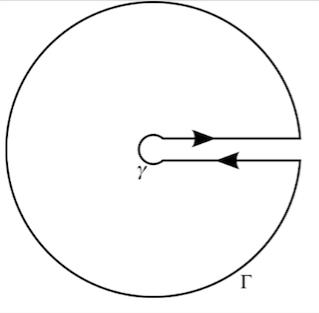
\includegraphics [scale=0.6] {keyhole.png} \end{center}
It's not labeled but the singularity $z_0$ is at the center of the two concentric circles.  The "keyhole" excludes $z_0$ so $f$ is analytic everywhere in the region enclosed by the path, and the total integral is zero by Cauchy's first theorem.  The straight line segments are so close as to be equal, but traversed in opposite directions, so the contribution from them is zero.  Thus we have that the integral around the outer ring counter-clockwise + the integral around the inner ring clockwise add up to zero.

Reversing the direction of integration on the inner ring changes the sign of the value, hence we have that
\[ \oint_{C \ \text{outer}} \frac{f(z)}{z-z_0} \ dz - \oint_{C \ \text{inner}} \frac{f(z)}{z-z_0} \ dz = 0 \]
But we haven't said anything about the radius of these rings.  

What this means is that the value of the integral around a ring enclosing a singularity is not zero, but it has the same value for a ring of \emph{any} radius.  It's independent of the radius.
\[ \oint_{C \ \text{outer}} \frac{f(z)}{z-z_0} \ dz = \oint_{C \ \text{inner}} \frac{f(z)}{z-z_0} \ dz \]

We can parametrize this path by saying that each point on the curve is given by
\[ z = z_0 + \rho e^{i\theta}, \ \ \ 0 \le \theta \le 2 \pi \]
\[ dz = \rho i e^{i \theta} \ d \theta \]
\[ \oint \frac{f(z)}{z - z_0} \ dz = \int_0^{2\pi} \frac{f(z_0 + \rho e^{i\theta})}{\rho e^{i \theta}} \ \rho i e^{i\theta} \ d \theta \]
\[ = i \int_0^{2\pi}  f(z_0 + \rho e^{i\theta}) \ d \theta \]
\[ = i \int_0^{2\pi}  f(z) \ d \theta \]
We may choose $\rho$ as small as we like, and in particular, if we choose it very small ($\rho \rightarrow 0$) we have
\[ f(z) \rightarrow f(z_0) = \text{constant} \]
and since it's constant we can bring it out of the integral!
\[  \oint \frac{f(z)}{z - z_0} \ dz = f(z_0) i \int_0^{2\pi} d \theta \]
\[ = 2 \pi i f(z_0) \]

In previous sections we derived three important theorems about complex functions.  (1) The Cauchy-Riemann equations (CRE) apply to analytic functions---functions that have derivatives---and vice-versa.
\[ u_x = v_y \]
\[ u_y = - v_x \]
We allow analytic functions to have a finite number of isolated singularities or poles where the function may "blow up."

(2) We used the CRE and Green's theorem to show that if a function is analytic everywhere in a simply-connected region, then the integral around any closed path in the region is zero.
\[ \oint f(z) \ dz = 0 \]
(3) On the other hand, if the region contains a singularity or pole, then we used a trick to show that the integral around \emph{any} closed path surrounding the pole has the same value.  This allows us to shrink the curve down to the immediate neighborhood of the pole and leads to the result in the limit as $z \rightarrow z_0$:
\[ \oint_C \frac{f(z)}{z - z_0} \ dz = 2 \pi i f(z_0) \]
(4) We can extend this result to a finite number of poles.  The value of the integral around all of them is the sum of the values for the individual poles.

\subsection*{example}
We can use the inverse function ($1/z$) as an example.  This function has a singularity at the origin.  Compare with the form of Cauchy2:
\[  \oint \frac{f(z)}{z - z_0} \ dz = 2 \pi i f(z_0) \]
We can match this form if we set $f(z) = 1$ and $z_0 = 0$.  The theorem says we can write the value of the integral as
\[ I = 2 \pi i f(z_0) = 2 \pi i \]
This matches what we obtained by parametrizing the unit circle.  There we had
\[ z = e^{i\theta}, \ \ \ \theta = 0 \rightarrow 2 \pi \]
\[ dz = iz \ d \theta \]
\[ \oint \frac{1}{z} \ dz = \int_0^{2\pi} i \ d \theta = 2 \pi i \]
This is $2 \pi i$ times the value of the function at $z_0 = 0$, which is $1$.

\subsection*{example}
Consider
\[ \oint \frac{6}{z(z-3)} \ dz \]
As shown in the figure, we are supposed to take for the curve $C$ the set of points $|z-3| = 5$, which is a circle of radius $5$ surrounding the point $z=3+0i$.
\begin{center} 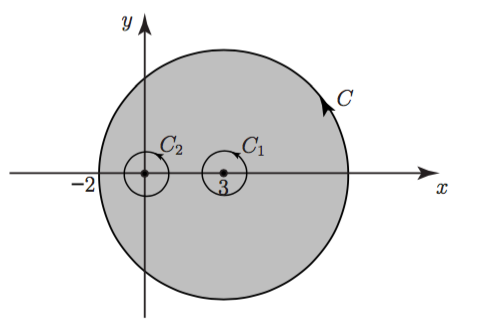
\includegraphics [scale=0.5] {cauchy2-fig1.png} \end{center}
This function does have two points of singularity, namely $z=0$ and $z=3$, so we expect that the value of the integral will not be zero.  We use (4) above to write
\[ \oint_C f(z) \ dz = \oint_{C_1} f(z) \ dz + \oint_{C_2} f(z) \ dz \]
We do not need to specify the curves because we will use (3) to calculate the values.

However, we do need to manipulate the function a bit.  We use the method of partial fractions.  Leaving aside the factor of $6$ for a moment:
\[ \frac{1}{z(z-3)} = \frac{A}{z} + \frac{B}{z-3} = \frac{A(z-3) + B(z)}{z(z-3)} \]
From looking at the numerator on the left- and right-hand sides, we see that $A = -B$ (because $Az + Bz = 0$), and that $-3A = 1$.  Hence
\[ A = -\frac{1}{3}, \ \ \ B = \frac{1}{3} \]
Recall the factor of $6$ and substitute for $A$ and $B$ in the middle expression to obtain:
\[ f(z) = \frac{-2}{z} + \frac{2}{z-3} \]
So now we can split the integrals for each curve into two parts.  We have:
\[ I = \oint_{C_1} f(z) \ dz + \oint_{C_2} f(z) \ dz \]
\[ = \oint_{C_1} \frac{-2}{z} \ dz + \oint_{C_1} \frac{2}{z-3} \ dz + \oint_{C_2} \frac{-2}{z} \ dz + \oint_{C_2} \frac{2}{z-3} \ dz  \]
Two of these four parts do not contain poles (the first and last), so those are just zero, and we have
\[ I = \oint_{C_1} \frac{2}{z-3} \ dz + \oint_{C_2} \frac{-2}{z} \ dz  \]
At this point we can use (3) from above, that
\[ \oint_C \frac{f(z)}{z - z_0} \ dz = 2 \pi i f(z_0) \]
(recognizing that the denominator for the second integral can be written as $z - 0$).  So the result is $2 \pi i f(z_0)$ for both integrals, but the value of the function is just $2$ for the first term and $-2$ for the second term, which cancel.  In this case, the total integral is just zero.
Notice that the cancellation comes because $A = -B$, which we would obtain for any two factors $z$ and $z - a$ ($a \ne 0$), as long as the function itself is a constant
\subsection*{example}
Consider
\[ \oint \frac{z}{z^2 + 1} \ dz \]
This function has poles at $z = \pm i$.
\begin{center} 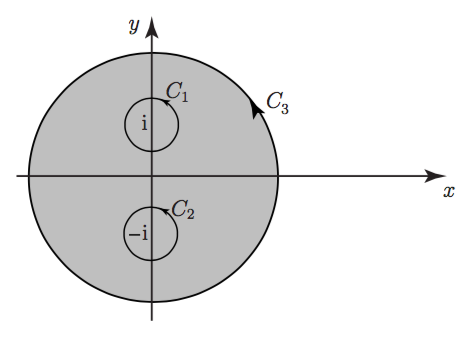
\includegraphics [scale=0.5] {cauchy2-fig2.png} \end{center}
We could find where the poles are by solving $z^2 + 1 = 0$ or we could factor
\[ z^2 + 1 = (z + i)(z - i) \]
This leads us to the strategy of partial fractions as before
\[ \frac{z}{z^2 + 1} = \frac{A}{z+i} + \frac{B}{z-i} \]
By inspection, $A = B = 1/2$ is a solution, so
\[ \oint \frac{z}{z^2 + 1} \ dz = \oint \frac{1/2}{(z+i)} + \frac{1/2}{(z-i)} \ dz  \]
As before, curve $C_1$ encloses a pole only for the second term, and $C_2$ for the first term.  We use
\[ \oint_C \frac{f(z)}{z - z_0} \ dz = 2 \pi i f(z_0) \]
where the function is simply the value $1/2$ at both points.  So we obtain
\[ 2 \pi i \  \frac{1}{2} = \pi i \]
for \emph{each} pole.

Another way is to write
\[ \frac{z}{z^2 + 1} = \frac{z}{(z + i)(z - i)} = \frac{z/z+i}{z-i} \]
For $C_1$, this has a pole at $z=i$, so the value of the integral is
\[ 2 \pi i \ f(z_0) = 2 \pi i \ \frac{i}{i+i} = \pi i \]
For $C_2$
\[  \frac{z/z-i}{z+i} \]
At the pole $z=-i$, the value of $f(z) = z/z-i$ is again $1/2$.

Yet another way to obtain this result, by analogy to calculus of real variables.  Substitute
\[ w = z^2 + 1 \]
\[ dw = 2 z \ dz \]
\[ \oint \frac{z}{z^2 + 1} \ dz = \frac{1}{2} \int \frac{1}{w} \ dw \]
\[ = \frac{1}{2} \ \text{Log} \ (w)   \]
\[ =  \frac{1}{2} \ \text{Log} \ (z^2 + 1)   \]
\[ \text{Log} \ z^2 = \text{Log} \ r^2 e^{i2\theta} = \ln r + 2 i \theta \]
if we evaluate over a closed contour ($\theta = 0 \rightarrow 2 \pi$) the terms with $\ln r$ vanish and we have then $4 \pi i$ times one-half or $2 \pi i$.
(Problem with the sum $+1$?

\subsection*{example}
\[ I = \int \frac{z^2}{4-z^2} \ dz \]
on the circle of radius $2$ centered at $z_0 = -1 + 0i$
\[ \gamma(\theta) = z_0 + 2e^{i \theta} = 1 + 2e^{i \theta} \]
Notice that the zeroes of the denominator occur at $z = \pm \ 2$ and that one of these is contained within our path of integration.

If we factor the denominator
\[ \frac{1}{4-z^2} = \frac{1}{4} \ [ \ \frac{1}{2-z} + \frac{1}{2+z} \ ] \]
we can split the integral
\[ I = \frac{1}{4} \int \frac{z^2}{2-z} + \frac{z^2}{2+z} \ dz \]
The first one is just zero, by Cauchy's theorem.  The second term contains the singularity:
\[ I = \frac{1}{4} \int \frac{z^2}{2+z} \ dz \]
Here $f(z) = z^2$ and 
\[ z - z_0 = z + 2 \]
so $z_0 = -2$ so the value of the manipulated integral is
\[ 2 \pi i \ f(z_0) = 2 \pi i \ 4 = 8 \pi i \]
and the value of the original one is
\[ I = \frac{1}{4} 8 \pi i = 2 \pi i \]

\section{Applications}
\subsection*{ellipse}
Karkhar gives this problem
\[ \int_0^{2\pi} \frac{1}{2 + \cos \theta} \ d \theta \]
Before we start I'd just point out that the equation for an ellipse in polar coordinates (with one focus at the origin) is
\[ r = \frac{b^2}{a - c \cos \theta} \]
If we neglect the minus sign (which just flips the orientation along the $x$-axis), let $a=2$ and $c=1$ and
\[ b^2 = a^2 - c^2 = 3 \]
rewrite
\[ \int_0^{2\pi} \frac{3}{2 + \cos \theta} \ d \theta \]
What this looks like to me is the integral of $r \ d \theta$ around an ellipse with $a = 2$ and $b = \sqrt{3}$.  This would be $r d \theta$ added up over the perimeter of that ellipse, i.e. the area.

Go back to the given problem.  Let
\[ z = e^{i\theta} \]
\[ dz = i z \ d \theta \]
\[ \cos \theta = \frac{1}{2}(e^{i\theta} + e^{-i \theta} ) \]
Use this result, but go back to $z$:
\[ \int_{|z|=1} \frac{1}{2 + (1/2)(z + 1/z)} \ \frac{1}{iz} \ dz \]
\[ = \frac{1}{i}  \int_{|z|=1} \frac{1}{2z + (1/2)(z^2 + 1)} \ dz \]
\[ = \frac{2}{i}  \int_{|z|=1} \frac{1}{z^2 + 4z + 1} \ dz \]
The roots of the denominator are $-2 \pm \ \sqrt{3}$.  One of these roots ($-2 + \sqrt{3}$) lies within our contour, which is just the unit circle.

Carry out partial fractions:
\[ \frac{1}{z^2 + 4z + 1} = \frac{A}{z - (-2 + \sqrt{3})} + \frac{B}{z - (-2 - \sqrt{3})} \]
\[ Az + A2 + A \sqrt{3} + Bz + B2 - B \sqrt{3} = 1 \]
Hence $A = -B$ and
\[ A2 + A \sqrt{3} -A2 + A \sqrt{3} = 1 \]
\[ 2A \sqrt{3} = 1 \]
\[ A = \frac{1}{2 \sqrt{3}} \]
The term we want is the one with $z_0 = (-2 + \sqrt{3})$ and that has coefficient $A$.  Hence the value is
\[ 2 \pi i \ (\frac{1}{2 \sqrt{3}}) = \frac{\pi i}{\sqrt{3}} \]
Pick up the leading factor of $2/i$ and obtain $2 \pi / \sqrt{3}$.

Going back to the argument about the ellipse at the beginning, multiplied by $3$ this gives $2 \sqrt{3} \pi$.  This is exactly the area of an ellipse with $a = 2$ and $b = \sqrt{3}$.

\subsection*{zz + 1}

This problem is Beck 4.26.  Consider 
\[ f(z) = \frac{1}{z^2 + 1} \]
We see that the denominator is zero when
\[ z^2 = -1, \ \ \ z = \pm \ i \]
Suppose our curve is the unit circle centered at $i$, designated as $C[i,1]$.  Obviously, this curve contains the singularity $z = i$.  Now
\[ z^2 + 1 = (z + i) (z-i) \]
Rewrite the function as
\[ f(z) = \frac{1/z+i}{z-i} \]
Then
\[ \int \frac{1}{z^2 + 1} \ dz = \int \frac{1/z+i}{z-i} \ dz \]
Cauchy's Integral formula says that
\[ f(w) = \frac{1}{2 \pi i} \ \oint  \frac{f(z)}{z-w} \ dz \]
The value of the function is
\[ \frac{1}{z+i}(i) = \frac{1}{2i} \]
and the integral in question is then.
\[ 2 \pi i f(w) = \pi  \]
\[ \int \frac{1}{z^2 + 1} \ dz = \pi \]

Similarly, if the unit circle is centered at $-i$, rewrite the function as
\[ f(z) = \frac{1/z-i}{z+i} \]
The value of the function is
\[ \frac{1}{z-i}(-i) = -\frac{1}{2i} \]
and that integral is then $- \pi$.

A contour that includes both singularities integrates to zero.

\subsection*{connection to reals}
Note that for the real function
\[ \int_0^{\infty} \frac{1}{1 + x^2} \ dx \]
We know the answer to this one, it is 
\[ \tan^{-1} x \ \bigg |_0^{\infty} = \frac{\pi}{2}  \]
Since $f(x)$ is an even function, the integral over $-\infty \rightarrow \infty = \pi$, and we feel there ought to be some connection between the two real and complex results.

Suppose we draw a part of the contour from $-\infty \rightarrow \infty$ on the real axis.  That integral is $\int f(z) \ dz$ but $y$ and $dy$ are both zero so it is just $\int f(x) \ dx$ with the result which we just obtained.

How to complete the contour?  Imagine the hemisphere in the upper half-plane with $R$ at $\infty$.  That is, parametrize
\[ \gamma(\theta) = Re^{i\theta}, \ \ \ \theta \in [0, \pi] \]
\[ \gamma \ '(\theta) =  iRe^{i\theta} \]
The integral is
\[ \int_0^{\pi} \frac{1}{1 + R^2 e^{i2\theta}} \ i R e^{i \theta} \ d \theta \]
Now what?
the 
It's clear that as $R \rightarrow \infty$, this integrand goes to 0.

\subsection*{example}

This problem is from wikipedia.  Consider
\[ g(z) = \frac{z^2}{z^2 + 2z + 2} \]
We want to evaluate the integral:
\[ I = \oint g(z) \ dz \]
The zeroes of the denominator are
\[ \frac{-2 \pm \ \sqrt{4-8}}{2} = -1 \pm \  \frac{\sqrt{-4}}{2} = - 1 \pm \ i \]
Confirm
\[ (z + (1 - i)) \ (z + (1 + i)) \]
\[ = z^2 + z + iz + z + 1 + i -iz - i + 1 \] 
\[ = z^2 + 2z + 2 \]
The denominator can then be rewritten as
\[ = \frac{A}{z + (1 - i)} + \frac{B}{z + (1 + i)}  \]
From the numerator we have
\[ A(z + (1 + i)) + B(z + (1 - i)) = 1 \]
So $A = -B$ and
\[ A(1 + i) + B(1 - i) = 1 \]
\[ A (1 + i) - A(1 - i) = 1 \]
\[ A 2i = 1 \]
\[ A = -\frac{1}{2i}, \ \ \ B = \frac{1}{2i} \]
The integral is
\[ \oint z^2 \ [ \ \frac{-1}{2i} \ \frac{1}{z + (1 - i)} + \frac{1}{2i} \ \frac{1}{z + (1 + i)} \ ] \ dz \]
If the contour is $|z| = 2$ (the circle of radius $2$, then both of the points lie within the contour.

We have two points
\[ z = -1 - i, \ \ \ z = -1 + i \]
We evaluate $2 \pi i f(z_0)$ for each and add them, where
\[ f(z) = -\frac{z^2}{2i} \]
\[ f(z_0) = -\frac{1}{2i} \ (-1 -i)^2 = -\frac{1}{2i} \ (1 + 2i -1) = -1 \]

for the first and for the second
\[ f(z) = \frac{z^2}{2i} \]
\[ = \frac{1}{2i} \ (-1 + i)^2 = \frac{1}{2i} (1 - 2i - 1) = -1 \]
Adding them together, the answer is just $I = -2 \times 2 \pi i = - 4 \pi i $.

\subsection*{example}
Consider
\[ \int_{\gamma} \frac{z^2}{4-z^2} \ dz \]
where $\gamma = | z + 1 | = 2$.
So the denominator of the function is
\[ \frac{1}{4-z^2} = \frac{1}{(2+z)(2-z)} \]
It has zeroes as $z = \pm \ 2$.  Only the point $z = 2$ is inside our contour.  So if we split this by partial fractions
\[  \frac{1}{(2+z)(2-z)} = \frac{1}{4} \ [ \ \frac{1}{2+z} + \frac{1}{2-z} \ ] \]
so we can rewrite the integral as
\[ I = \int_{\gamma} \frac{z^2}{4} \ [ \ \frac{1}{2+z} + \frac{1}{2-z} \ ] \ dz \]

By Cauchy's Theorem, the first term is zero.  The second one is:
\[ I = \int_{\gamma} \frac{z^2}{4} \ ( \frac{1}{2-z} ) \ dz \]
and the value of $I$ is
\[ I = 2 \pi i f(z_0) \]
where 
\[ f(z_0) = \frac{z^2}{4}  \ \bigg |_{z_0 = 2} = 1 \]
so the integral is just $2 \pi i$.

\subsection*{Karplan rules}
Kaplan gives some rules for computing residues:

\textbf{RULE I}  At a simple pole $z_0$ (that is, a pole of first order),
\[ \text{Res } [f(z),z_0] = \lim_{z \rightarrow z_0} (z-z_0) f(z) \]
\subsection*{example}
\[ f(z) = \frac{1}{z^2 + 1} = \frac{1}{(z - i)(z + i)} \]
\[ \text{Res } [f(z),z=i] = \lim_{z \rightarrow i} (z-i) \frac{1}{(z - i)(z + i)} \]
\[ = \lim_{z \rightarrow i} \frac{1}{z + i} = \frac{1}{2i} \]
\textbf{RULE II}  At a pole of order $N$ ($N = 2, 3, \dots$),
\[ \text{Res } [f(z),z_0] = \lim_{z \rightarrow z_0} (z-z_0) \frac{g^{(N-1)}(z)}{(N-1)!} \]
where 
\[ g(z) = (z-z_0)^N f(z) \]
\subsection*{example}
\[ f(z) = \frac{e^z}{z(z-1)^2} \]
We have a pole of first order at $z=0$ and one of second order at $z=1$.  At the first
\[ \text{Res } [f(z),z=0] = \lim_{z \rightarrow 0} \frac{e^z}{(z-1)^2} = 1 \]
For the other one, remove the factor of $(z-1)^2$ and compute the $N-1$ (first) derivative of what's left
\[ \text{Res } [f(z),z=1] = \lim_{z \rightarrow 1} \ [ \ \frac{e^z}{z} \ ]' \ \]
\[ = \frac{e^z z - e^z}{z^2} \ \bigg |_1 =  0 \]
Hence
\[ \oint f(z) \ dz = 2 \pi i \ [ \ \sum  \text{Res } \ ] \ = 2 \pi i \]
\textbf{RULE III}  If $A(z)$ and $B(z)$ are analytic in a neighborhood of $z_0$, $A(z_0) \ne 0$, and $B(z)$ has a zero at $z_0$ of order 1, then
\[ f(z) = \frac{A(z)}{B(z)} \]
has a pole of first order at $z_0$ and
\[ \text{Res } [f(z),z_0] = \frac{A(z_0)}{B'(z_0)} \]
\subsection*{example}
\[ f(z) = \frac{1}{z^2 + 1} = \frac{1}{(z - i)(z + i)} \]
\[ B = z^2 + 1, \ \ \ B' = 2z \]
\[ \text{Res } [f(z),z=i] = \frac{1}{2i} \]
\[ \text{Res } [f(z),z=-i] = -\frac{1}{2i} \]
\subsection*{example}
\[ f(z) = \frac{z e^z}{z^2 - 1} \]
Both top and bottom are analytic.  The poles of $B(z)$ are at $\pm \ 1$.  $A(z) \ne 0$ at those points.  We have 
\[ \frac{A(z)}{B'(z)} = \frac{z e^z}{2z} \]
\[ \frac{z e^z}{2z} \ \bigg |_{z=1} = \frac{e}{2} \]
\[ \frac{z e^z}{2z} \ \bigg |_{z=-1} = e^{-1} \]
\textbf{RULE IV}  If $A(z)$ and $B(z)$ are analytic in a neighborhood of $z_0$, $A(z_0) \ne 0$, and $B(z)$ has a zero at $z_0$ of order 2, then
\[ \text{Res } [f(z),z_0] = \frac{6A' B'' - 2AB'''}{3B''^2} \]
\subsection*{example}
\[ f(z) = \frac{e^z}{z(z-1)^2} \]
\[ B = z(z^2 - 2z + 1) = z^3 - 2z^2 + z \]
\[ B' = 3z^2 - 4z + 1 \]
\[ B'' = 6z - 4 \]
\[ B''' = 6 \]
So
\[ \frac{6A' B'' - 2AB'''}{3B''^2} = \frac{6(e^z)(6z-4) - 2e^z(6)}{3(6z-4)^2} \ \]
Evaluate at $z=1$:
\[ \frac{6e(2) - 2e(6)}{12} = 0 \]
So only the pole at $z=0$ contributes.


\end{document} 